After a comprehensive proposal for a cooperative perception system, including a novel modeling approach and an elaborate distributed software architecture, was presented in the previous chapters, this chapter aims to evaluate the system with respect to different aspects.

\Cref{sec:problem_analysis:goals_requirements} presented a set of goals and requirements to be met by the proposed system. While previous chapters already discussed how most of them are individually addressed, a few demand for further investigation or empirical assessment. Accordingly, a two-fold evaluation is conducted. The first part concerns with evaluating the proposed \textbf{software architecture} in terms of performance, specifically with respect to the requirements of scalability (NF-C2) and efficiency (NF-C3). The second part of the evaluation aims to assess the system's qualitative \textbf{performance in cooperative perception} tasks, motivated by the overall goal of this thesis to facilitate the improvement of connected, autonomous vehicles' average perception quality (cf. \cref{sec:problem_analysis:goals_requirements}). Both parts are split into three or sections each, that describe the respective evaluation's specific goal and methodology, present the results and eventually discuss them in a brief conclusion.

\section{Performance Evaluation}
\label{sec:evaluation:performance_evaluation}
\Cref{sec:problem_analysis:goals_requirements} stated the non-functional requirements for the system to be able to handle 202 concurrent network participants at minimum and to aim for low latency and on-vehicle load. The following evaluation thoroughly assesses the previously developed system with respect to both criteria, i.e. \textbf{system scalability} and \textbf{communication efficiency}.

\subsection{Methodology}
\label{subsec:evaluation:performance_evaluation:methodology}
First, one or more metrics need to be determined with respect to which the evaluation of the above criteria should be conducted. With regards to scalability, a precise quantity is given as a requirement, which refers to the number of concurrent clients (i.e. vehicles, pedestrians, etc.) the system is expected to handle at minimum. Assuming a fixed per-vehicle message publish rate – which is in accordance with the previously introduced \textit{periodic push} principle – this translates to a \textbf{minimum number of observation messages (Q1)}, i.e. state representations, the edge node must be able to process at a time. While the concrete message rate is a parameter that can be varied over the course of the evaluation, a hard minimum requirement of 202 concurrent vehicles is given. That is, assuming the entire system to operate at \SI{10}{Hz} (i.e. both client- and server-side publish rate), the fusion node must reliably process 2020 observations per second without dropping below that rate. In addition, average \textbf{latency in milliseconds (Q2)} and average \textbf{message size in kilobytes (Q3)} per vehicle and per observation are to be determined to cover communication efficiency. Latency, in this specific context, refers to the average delay of a shared observation until received by an ego vehicle and can generally be thought of the average "'outdatedness"' of a CP message.
\par
\bigskip

Message size (Q2) is constant per vehicle and its determination can be done trivially by inspecting and aggregating the individual sizes of incoming messages at the fusion node without any special setup. For better comparison, an additional boolean parameter \texttt{WITH\_OCCUPANT} is introduced to denote whether or not an occupancy cell should include information about its potential occupant in addition to its pure state.
\par
\bigskip

Concerning the latency (Q3), we are primarily interested in how it is composed. Instead of trying to estimate total latency as a function of traffic density / number of network participants, we rather want to get insights about which parts of the fusion process are the most temporally critical ones to help later optimization of certain system components and functions. Accordingly, the relative durations $d_{i \in [0..6]}$ between relevant instants $t_{j \in [0..7]}$ of the fusion process, schematically depicted in \cref{fig:communication_timeline}, are to be determined for a fixed parameter configuration in an ordinary setup. To help that, existing code is extended in various placed across Talky edge node and Talky client to add time measuring functionality.
\par
\bigskip

\begin{figure}[h]
	\centering
	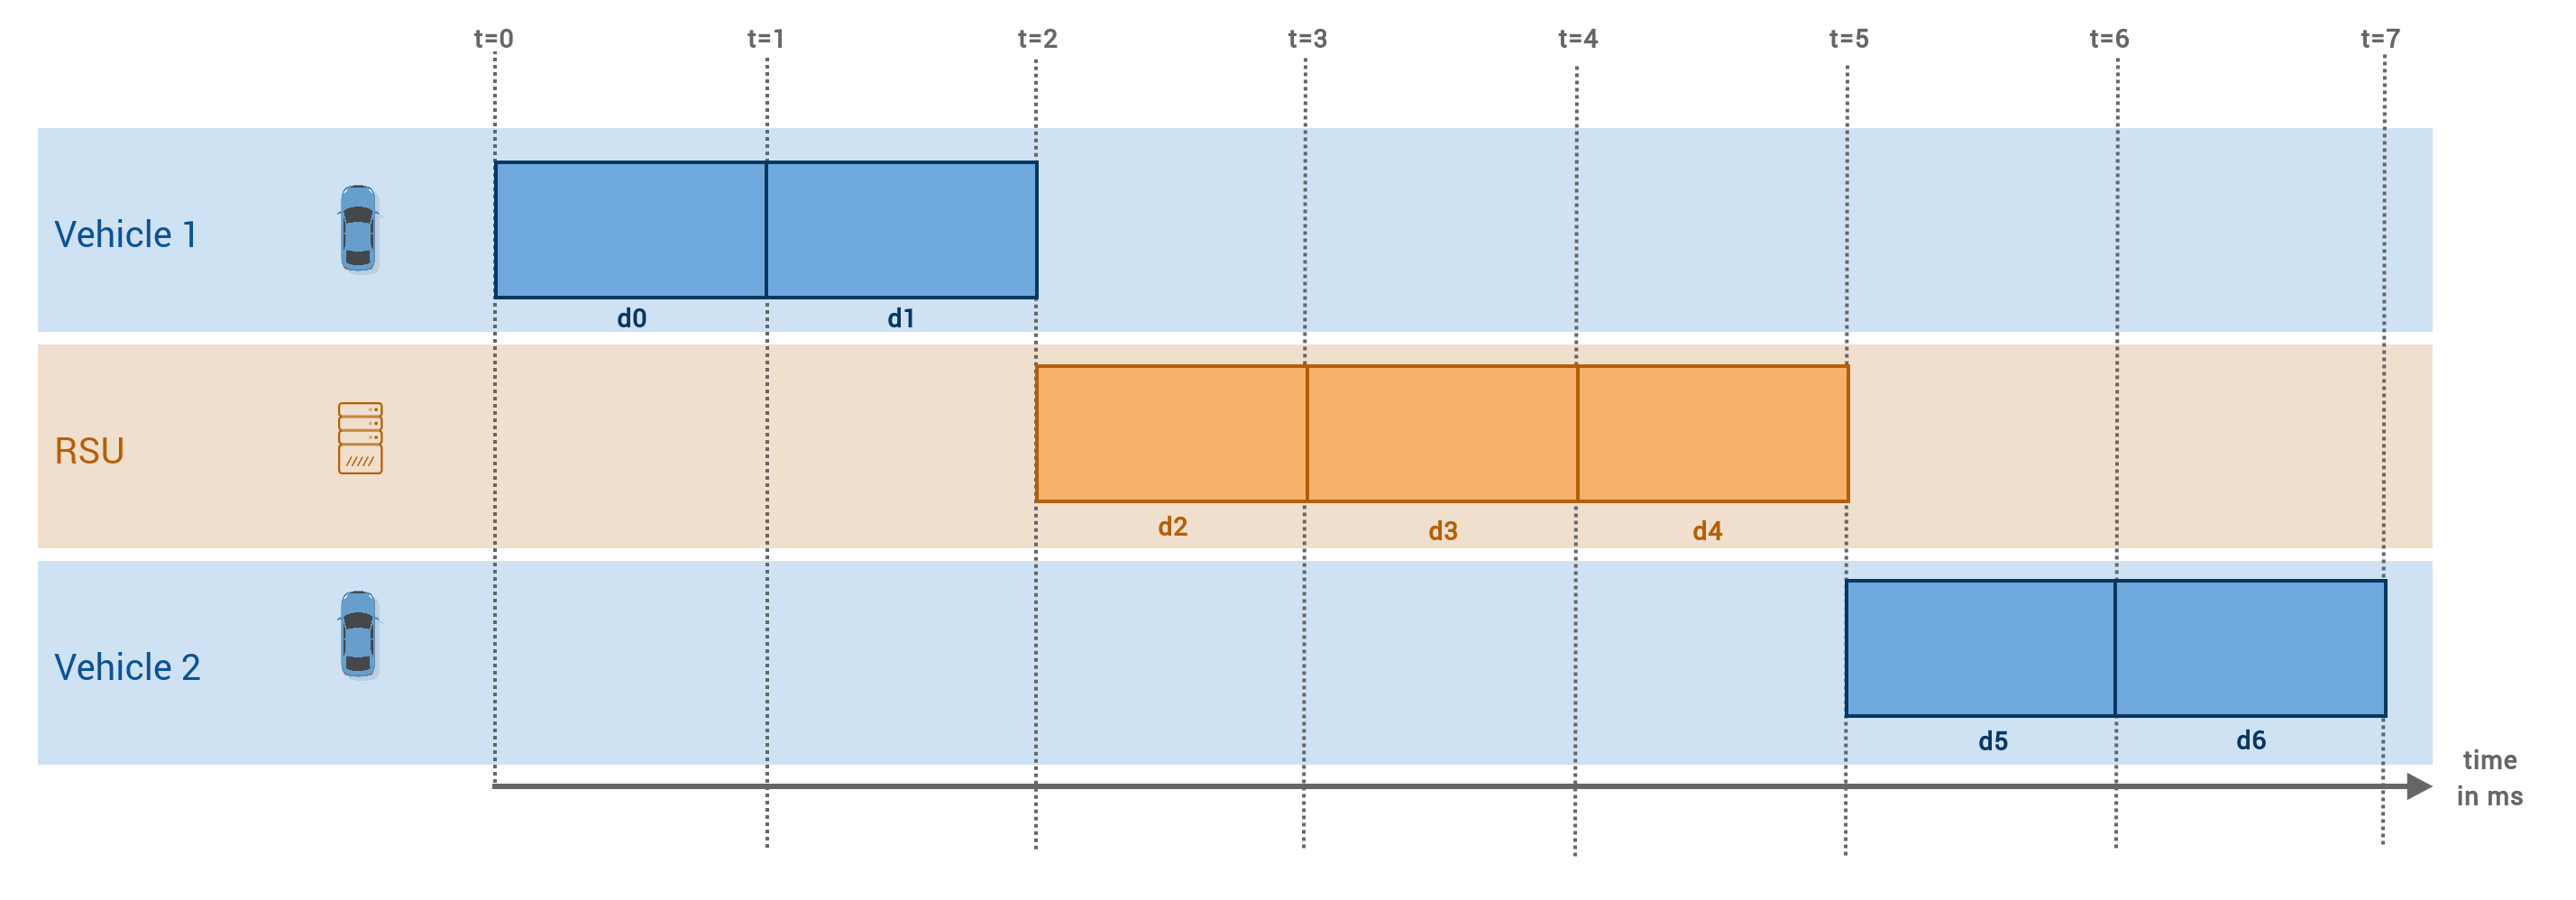
\includegraphics[width=1\linewidth]{98_images/communication_timeline}
	\caption{Timing Composition of Fusion Process}
	\label{fig:communication_timeline}
	\medskip
	\small
	\begin{enumerate}[t = 1:\ ]
		\item An observation is obtained by local sensory and low-level fusion (including ray casting-facilitated cell matching, etc., cf. \cref{subsec:implementation:talky_client}) \\
		\item The observation is encoded locally, i.e. represented as a PER model and serialized to Protobuf format
		\item The observation is received remotely, i.e. at the fusion node
		\item The observation is decoded remotely, i.e. deserialized from Protobuf and converted to process-local data structures
		\item The observation is remotely fused with other relevant observations from different observers, encoded to a PER model instance and serialized to Protobuf again
		\item The fused observation is received locally by the ego vehicle
		\item The fused observation is decoded locally
	\end{enumerate}
\end{figure}

In order to gather (Q1), a minimalist sub-system of the entire CP software system is employed. It still follows a client-server architecture and has the message broker and fusion node on one end and multiple (simulated) ego vehicles on the other. Since we are only interested in quantitative measurements rather than in the messages' actual content, a newly created message generator program is used to artificially simulate observations instead of employing an actual Carla simulation with real Talky clients. Otherwise it would be infeasible to test with a large number of vehicles, due to exceedingly high computation load. The multi-threaded message generator is parameterized with (1) the target size of the generated occupancy grid observations, (2) the number of concurrent clients to simulate and (3) a per-client frequency at which to push messages to the backend (see \cref{tab:performance_evaluation:variable_parameters}). Moreover, supplementary code is added to the fusion node to track how often the \texttt{Publish()} method is called.

The test setup involves two physical machines, interconnected via a \SI{1}{\giga\bit\per\second} Ethernet network. One machine (AMD Ryzen 1600 \SI{3.2}{\giga\hertz} 6-core CPU, \SI{16}{\giga\byte} RAM, Ubuntu 18.04) runs the backend part of the system, i.e. message broker and edge node, while the message generator is run on the other (Intel i5-6600K \SI{4.5}{Ghz} 4-core CPU, \SI{16}{\giga\byte} RAM, Manjaro 18.1).
\par
\bigskip

\Cref{tab:performance_evaluation:constant_parameters} lists all fixed parameters used for the entire evaluation. Parameters marked with a star (*) are mentioned for completeness, but should not have any influence on the measured quantity. For the experiment, randomly generated occupancy grids lie within the same type 3 tile are used in the observation messages. \Cref{tab:performance_evaluation:variable_parameters} lists all variable, evaluation-specific parameters to be tested in order to get insights about their respective impact on the final results. To test all combinations of parameters for investigating (Q1), a grid search is conducted, i.e. a test is run for every combination in the Cartesian space of parameter values. For (Q2) and (Q3) only a single parameter set $\vartheta = \{ \texttt{N\_EGOS} = 6, \texttt{OBSERVATION\_RATE} = 10, \texttt{GRID\_RADIUS} = 11 \}$ is used.

\begin{table}
	\centering
	\begin{tabular}{|p{4.5cm}|p{2cm}|}
		\hline 
		\textbf{Parameter} & \textbf{Value} \\ \hline 
		\texttt{TILE\_1\_LEVEL} & \texttt{24} \\ \hline 
		\texttt{TILE\_2\_LEVEL} & \texttt{19} \\ \hline 
		\texttt{TILE\_3\_LEVEL} (*) & \texttt{15} \\ \hline 
		\texttt{MQTT\_QOS} & \texttt{1} \\ \hline 
		\texttt{DECAY\_FACTOR} (*) & \texttt{0.11} \\ \hline 
		\texttt{FUSION\_RATE} (*) & \texttt{10} \\ \hline 
		\texttt{OBSERVATION\_MAX\_AGE} & \texttt{3600} \\ \hline 
		\texttt{WITH\_OCCUPANT} & \texttt{false} \\ \hline 
	\end{tabular}
	\caption[Constant Parameters of the Performance Evaluation]{Constant Parameters of the Performance Evaluation. See \cref{sec:implementation:configurable_parameters} for descriptions.}
	\label{tab:performance_evaluation:constant_parameters}
\end{table}

\begin{table}
	\centering
	\begin{tabular}{|p{3.5cm}|p{8.5cm}|p{3.2cm}|}
		\hline 
		\textbf{Paremeter} & \textbf{Description} & \textbf{Values} \\ 
		\hline 
		\texttt{N\_EGOS} & Numbers of concurrent simulated clients exchanging CP messages & \texttt{\{25, 50, 75, 100, 200, 400, 800, 1600\}} \\ 
		\hline 
		\texttt{OBSERVATION\_RATE} & Frequency at which observations are periodically published to the network by each of its participants & \texttt{\{1, 5, 10\}} \\ 
		\hline 
		\texttt{GRID\_RADIUS} & Occupancy grid radius in number of cells. With $\lambda_1 = 24$ these are approx. equal to a grid size (i.e. observation range) of \texttt{\{52.8, 100.8\}} meters & \texttt{\{11, 21\}} \\ 
		\hline 
	\end{tabular}
	\caption{Variable Parameters of the Performance Evaluation}
	\label{tab:performance_evaluation:variable_parameters}
\end{table}

In summary, two steps are performed to gather the above metrics. First, to find (Q1), multiple iterations – each according to one parameter set – are run using the minimal system subset in the presented two-machine setup. Second, the entire CP system including a Carla simulation instance is run in a single machine to obtain (Q2) and (Q3) for a fixed parameter set. 

\subsection{Results}
\label{subsec:evaluation:performance_evaluation:results}
In accordance with the structure presented in the previous section, results are obtained in two steps.
\par
\bigskip

First, a set of experiments are conducted to get insights about the Talky edge node's \textbf{maximum fusion rate (Q1)}, depending on three different parameters. While most parameters, including the edge node's fusion rate, are fixed at a certain value (see \cref{tab:performance_evaluation:constant_parameters}), the number of concurrent network participants and their publishing frequency and grid size are varied. Consecutively executing the evaluation with a total of 30 different configurations yields the results depicted in \cref{fig:performance_evaluation:fusion_rates}.

\begin{figure}
	\centering
	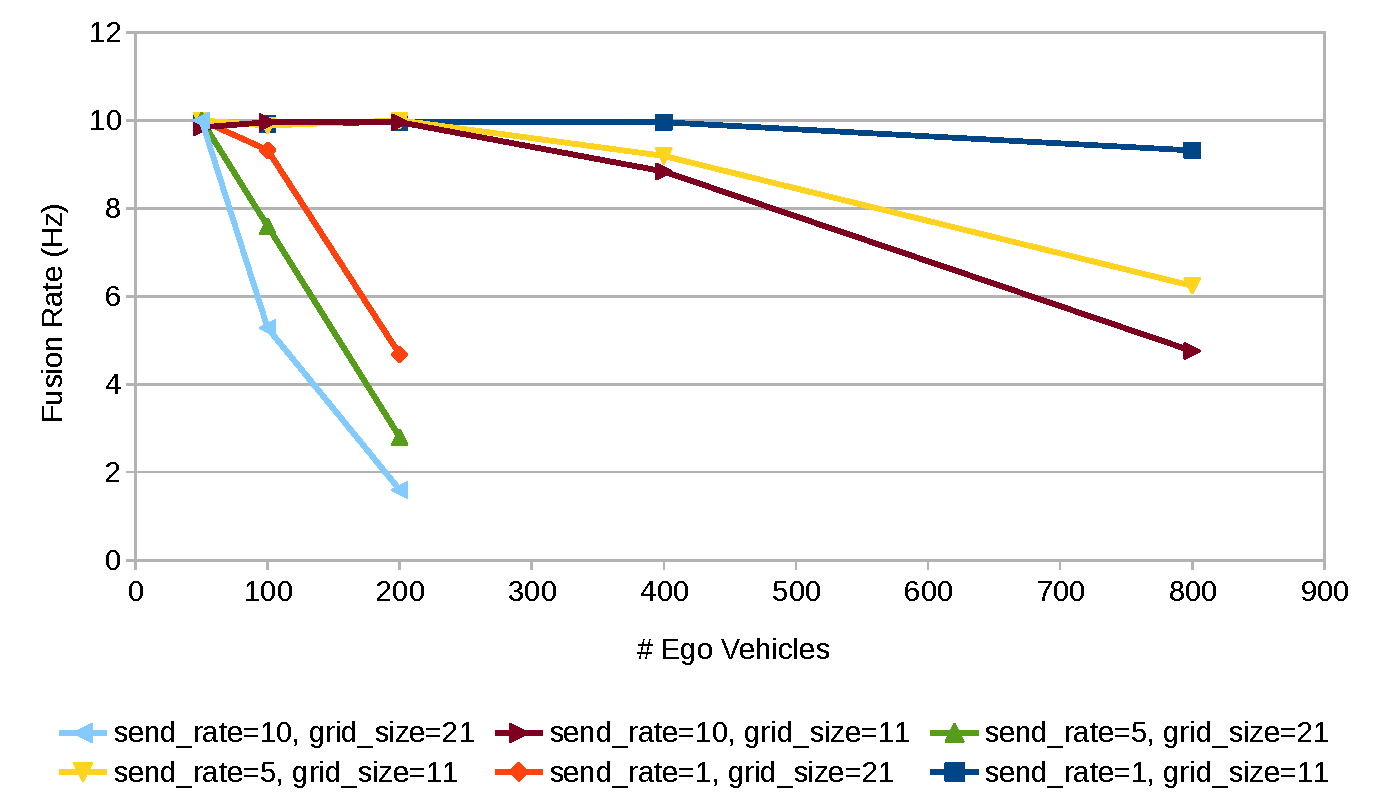
\includegraphics[width=1.0\linewidth]{98_images/performance_evaluation_chart1}
	\caption{Average Measured Fusion Rate}
	\label{fig:performance_evaluation:fusion_rates}
\end{figure}

It can be seen that the maximum possible fusion rate heavily depends on both the incoming message rate and the occupancy grids' size. While the fusion node is able to maintain a rate of \SI{10}{\hertz} for up to nearly 800 concurrent vehicles if their observation range is $\sim$ \SI{52.8}{\meter} (11 by 11 cells at $\lambda_1 = 24$), it tends to drop below that threshold as observation rate and grid size increase. Assuming a fusion rate of \SI{10}{\hertz}, the hard requirement of being able to handle $\sim$ 200 concurrent vehicles can only be fulfilled with the smaller observation range of \texttt{GRID\_RADIUS=11}, regardless of the client's publish frequency. If the client vehicles are expected to publish their environment observations from a range of $\sim$ \SI{100.8}{\meter} instead, the current Talky edge node implementation would not be able to keep up at a fusion rate of \SI{10}{\hertz}. However, if the system's fusion rate is lowered to, for instance, \SI{5}{\hertz} – which is still not an unrealistic value – the fusion node could fulfill the requirement for all test scenarios. As an additional excursus, the MQTT broker's performance is evaluated separately to eliminate the possibility of it constituting a bottleneck to the system. However, using the \texttt{mqtt-bench}\footnote{\url{https://github.com/takanorig/mqtt-bench}} benchmarking tool, it was found that Mosquitto (version 1.6.8) is able to handle up to \SI{8000}{messages\per\second} with a message size of \SI{12}{\kilo\byte} (approximately corresponding to 11x11-cell grids, see \cref{tab:performance_evaluation:message_sizes}) and up to \SI{4100}{messages\per\second} with a message size of \SI{46}{\kilo\byte} (21x21-cell grids). Therefore, the broker only becomes a limiting factor with more than 800 or 410 concurrent vehicles respectively. The benchmark results can be found in \cref{sec:appendix:evaluation_results:mqtt_broker_benchmark}.
\par
\bigskip

In a second step, average message size latency are investigated. Results for the former are depicted in \cref{tab:performance_evaluation:message_sizes}. The minimum achievable \textbf{average message size (Q2)} of a Protobuf-serialized PER model instance was found to be \SI{12}{\kilo\byte} (\SI{46}{\kilo\byte}) with a grid radius of 11 cells (21 cells), corresponding to an observation range $\sim$ \SI{52.8}{\meter} (\SI{100.8}{\meter}). Such minimalist model instances contain nothing but the observer information, the occupancy grid and an estimated state value for each cell. When including additional information about the occupant (vehicle, pedestrian, static obstacle, etc.) of a cell, the average message size increases accordingly.

\begin{table}
	\centering
	\begin{tabular}{|p{6.2cm}|p{3.5cm}|p{3.5cm}|}
		\hline 
		& \texttt{GRID\_RADIUS = 11} & \texttt{GRID\_RADIUS = 21} \\ 
		\hline 
		\texttt{WITH\_OCCUPANT = false} & \SI{12}{\kilo\byte} & \SI{46}{\kilo\byte} \\ 
		\hline 
		\texttt{WITH\_OCCUPANT = true} & \SI{32}{\kilo\byte} & 1\SI{21}{\kilo\byte} \\ 
		\hline 
	\end{tabular}
	\caption[Average Measured Observation Message Sizes]{Average  Measured Observation Message Sizes (occupied cells)}
	\label{tab:performance_evaluation:message_sizes}
\end{table}
\par
\bigskip

As a result of investigating how an observations total \textbf{latency (Q3)} is composed in the present CP system, the duration values presented in \cref{tab:performance_evaluation:latency_composition} were observed. Instants and durations shown in the table refer to those presented in \cref{fig:communication_timeline}. As can be seen in the table, two separate, but related time series were measured for completeness. While the first includes an entire round trip, the second excludes $t=0$ and starts at instant $t=1$, i.e. at the moment a local observation is already present. With respect to the evaluation goal, this is more meaningful, as it only measures the actual CP process and disregards observer-specific performance of local perception and low-level sensor fusion. In our experiments, a globally fused observation is on average \SI{289}{\milli\second} old when it arrives at a client again. In other words, given the system runs at \SI{10}{\hertz} it takes \SI{289}{\milli\second} for a local observation to take the journey from a vehicle over the message broker and Talky edge node back to a vehicle. However, two key points must be kept in mind when interpreting these results. First, an local area network (LAN) with Ethernet was used instead of cellular 5G. Second, some of the depicted duration values include an "'idle"' delay caused by the fact that the system runs at a fixed rate (\SI{10}{\hertz} in this case). For instance, when an observation is received at the fusion node, it takes, on average $\mu_{\delta t} = \frac{1}{2} * \frac{\SI{1}{\second}}{10} = \frac{1}{2} *  \SI{100}{\milli\second} = \SI{50}{\milli\second}$ to get "'picked up"' by the fusion routine. After normalizing the duration values by this average delay (denoted in brackets in \cref{tab:performance_evaluation:latency_composition}), it can be seen that receiving an observation locally ($t_4 \rightarrow t_6 = d_5$) takes longest, although receiving it remotely is much faster ($t_2 \rightarrow t_3 = d_2$). This might potentially be caused by a "'queuing"' effect resulting from poor performance of the client-side message processing, but demands for further investigation in future work. Local encoding (model instantiation and Protobuf serialization) ($t_1 \rightarrow t_2 = d_1$) makes up another significant part of the total latency, but is still faster than with the previous approach of using Cap'n'Proto (cf. \cref{subsec:implementation:serialization_format}). Overall, the average total delay of \SI{289}{\milli\second} (\SI{189}{\milli\second} normalized) can be considered acceptable, especially given that the current implementation is rather a proof-of-concept than an optimized system solution. However, further research is required to investigate latency in real-world scenarios and using actual cellular networks.

\begin{table}
	\centering
	\begin{tabular}{|p{1.5cm}|p{4.1cm}|p{4.1cm}|p{4.1cm}|}
		\hline 
		\textbf{Instant} & \textbf{Time Offset} (with local perception) & \textbf{Time Offset} (without local perception) & \textbf{Duration} ($t_{i-1} \rightarrow t_i$) \\ 
		\hline 
		\textbf{t=0} & \SI{0}{\milli\second} & – & – \\ 
		\hline 
		\textbf{t=1} & \SI{260}{\milli\second} & \SI{0}{\milli\second} & \SI{260}{\milli\second} \\ 
		\hline 
		\textbf{t=2} & \SI{288}{\milli\second} & \SI{28}{\milli\second} & \SI{28}{\milli\second} \\ 
		\hline 
		\textbf{t=3} & \SI{341}{\milli\second} & \SI{81}{\milli\second} & \SI{53}{\milli\second} (\SI{3}{\milli\second}) \\ 
		\hline 
		\textbf{t=4} & \SI{343}{\milli\second} & \SI{83}{\milli\second} & \SI{2}{\milli\second} \\ 
		\hline 
		\textbf{t=5} & \SI{501}{\milli\second} & \SI{241}{\milli\second} & \SI{58}{\milli\second} (\SI{8}{\milli\second}) \\ 
		\hline 
		\textbf{t=6} & \SI{545}{\milli\second} & \SI{285}{\milli\second} & \SI{44}{\milli\second} \\ 
		\hline 
		\textbf{t=7} & \SI{549}{\milli\second} & \SI{289}{\milli\second} & \SI{4}{\milli\second} \\ 
		\hline 
	\end{tabular}
	\caption{Cooperative Perception Latency Composition}
	\label{tab:performance_evaluation:latency_composition}
	\medskip
	\small
	Durations are additionally normalized with the expected delay of $\mu_{\delta t} = \SI{50}{\milli\second}$ caused by periodic push at \SI{10}{\hertz}
\end{table}
\par
\bigskip

A further discussion about the implication of any of these results is done in the next section. 

\subsection{Discussion \& Conclusion}
\label{subsec:evaluation:performance_evaluation:discussion_conclusion}
With respect to scalability, it was shown that a single Talky fusion node is able to fulfill the requirement of handling more than 202 concurrent clients with an observation range of $\sim$ \SI{50}{\meter} up to a fusion rate of \SI{10}{\hertz}. Given a \SI{100}{\meter} observation range, the system would at least be able to support \SI{5}{\hertz}. While the authors if \cite{Calvo2017} suggest to run their system at \SI{10}{\hertz}, \cite{Thandavarayan2019} showed that certain optimizations can decrease the required message rate for cooperative perception to \SI{4.5}{\hertz} without sacrificing perception quality. Hence, the present prototype system's performance can be considered acceptable, although there is large room for optimizations. Such include the following.

\begin{itemize}
	\item Algorithmic optimizations of the fusion routine: the current implementation has superlinear complexity and might potentially be reworked to scale better. For instance, Petrich et al. \cite{Petrich2018} showed that a relational traffic scene representation – like the present PER model – can be transformed to a \textbf{tensor format}, which potentially enables for fusion to be represented as matrix operations. Such can be run on a GPU in a highly optimized fashion and potentially boost performance by orders of magnitude. Another potentially promising optimization is to extend the current, naive fusion to \textbf{probabilistic fusion}, which is a concept that, to the best of our knowledge, no previous work had covered, yet. The basic idea here is to sample a smaller subset of all available observations using a particular probability distribution, so that the entire spatial area is still best represented in the sample. 
	\item Parameter optimization: for the sake of simplicity, only a very small set of different parameters were tested in the previous evaluation. However, for real-world deployment, one would want to thoroughly \textbf{determine optimal values} for any of the parameters presented in \cref{sec:implementation:configurable_parameters}. For instance, the authors of \cite{Gunther2015} run their CP system at only \SI{1}{\hertz} and with a communication range of \SI{300}{\meter} (compared to \SI{611}{\meter} or \SI{1223}{\meter} in our experiments). This holds potential to dramatically improve performance.
	\item Message generation optimizations: \cite{Thandavarayan2019} presents a rich set of thought on how to \textbf{optimize the generation and publishing} of CPMs. For instance, the authors worked out sophisticated heuristics to determine when a message would contain enough valuable information about the current to be published and when it is better hold back for another few time steps. In complement to that, \cite{Breu2013} presents a way to efficiently \textbf{estimate the relevance} of a CAM for its recipient, mainly based on the sender and recipient's trajectory.
\end{itemize}
\par
\bigskip

With respect to communication efficiency, our evaluations found that, given a per-vehicle observation range of $\sim$ \SI{50}{\meter}, the average message size ranges from \SI{12}{\kilo\byte} without occupant information to \SI{32}{\kilo\byte} with such. Naively assuming an available bandwidth of \SI{200}{\mega\bit} (cf. \cref{subsec:concept_design:5g_usage_scenarios_advantages}), the network could handle $\sim$ 2080 or 780 messages per second respectively. Without conducting a more elaborate estimation, this can generally not be considered sufficient. Accordingly, the format of exchanged messages would have to undergo further optimization in the future. Such optimizations might include server- and client-side \textbf{caching} of de-facto constant properties of actors, e.g. the \texttt{boundingBox} of a \texttt{DynamicObstacle} used within an \texttt{observedBy} relation of an \texttt{OccupancyGrid} (see \cref{subsec:concept_design:the_final_model}). In addition, the cells of an occupancy grid can be represented more efficiently by only transmitting the top-left and bottom-right cell's hash, instead of all, since that information is redundant. Moreover, the optimization methods (e.g. with regard to message generation) mentioned above apply to improving communication efficiency likewise.

As a result to investigating a CP iteration's total latency and how it is composed, an average "'outdatedness"' of shared observations of $\sim$ \SI{289}{\milli\second} was found, when disregarding the local measuring process. Whether or not this is a suitable delay for a CP system is discussed in the next \cref{sec:evaluation:perception_evaluation}.

\section{End-to-end Perception Evaluation}
\label{sec:evaluation:perception_evaluation}
This part of the evaluation analyzes the proposed system's cooperative perception performance in and end-to-end fashion. Goal is to determine to what degree autonomous connected cars can improve their perception quality through cooperatively sharing their local belief about the environment. While the performance evaluation in \cref{sec:evaluation:performance_evaluation} examined certain characteristics of the system itself, in this part it is rather viewed as a black box to measure its impact end to end. 
\par
\bigskip

Different approaches can be taken to measure overall CP performance. For instance, the authors of \cite{liu2013motion} evaluate their system with regard to planning. More specifically, they compare the smoothness or "'jerk"' of an automated vehicle's generated trajectories with and without cooperation. Another way is presented in \cite{Chen2019}. In this case, the authors evaluate their low-level fusion-based system with regard to detection range and confidence, i.e. they measure the percentage and distance of detected obstacles alongside the average observation confidence with and without CP respectively. The approach taken by this evaluation is similar to the latter and focuses on perception / detection rather than on planning. Given multiple automated, connected cars in a simulation, goal is to observe the \textbf{overall average perception quality improvement} in terms of detection accuracy and confidence. As a part of that, we also investigate how this potential improvement is impacted by the \textbf{observer network's density} and different parameter values for \textbf{temporal decay}.

\subsection{Methodology}
\label{subsec:evaluation:perception_evaluation:methodology}

\subsubsection{Idea \& Structure}
The present evaluation is structured into three closely related parts. First, the proposed system's \textbf{general suitability} (\textbf{Part 1}) for cooperative perception tasks is assessed, i.e. goal is to determine the extent to which perception quality can be improved through cooperation. Subsequently, it is further investigated how this potential improvement is affected by the \textbf{number of connected, communicating vehicles (Part 2)} and by different \textbf{temporal decay factors (Part 3)} (see \cref{subsec:concept_design:fusion_mechanism}). As mentioned earlier, the evaluation is conducted in an end-to-end fashion in the sense that measurements taken in multiple simulated scenarios are accumulated and viewed as a whole, rather than looking into particular aspects of the system itself. The setup is as follows.
\par
\bigskip

A variable number of ego vehicles are simulated in a pre-defined Carla environment. Each of these comprise an instance of the client-side parts (cf. \cref{subsec:concept_design:components_overview}) of the previously developed CP system and are connected to a centrally deployed instance of the respective server-side part, i.e. message broker and fusion node. Given pseudo-randomly \textbf{generated start- and destination} waypoints on the Carla map, they automatically traverse their environment while facing pseudo-randomly placed static and dynamic obstacles, such as other traffic participants. While doing so, their observations in the form of PER model instances, each of which contains an occupancy grid and respective cell state estimations, are recorded for later analyses. Multiple different scenarios are consecutively tested, in each of which static obstacle positions and start- and destination points of dynamic obstacles and ego vehicles are varied. Every configuration is run multiple times to later calculate an average score. The key point of this evaluation is to "'virtually"' \textbf{run each set of experiments twice} in addition: once with the Talky fusion node \textbf{turned on and off} respectively, i.e. with the ego vehicles communicating with each other or not. Subsequently, both result sets are compared to learn whether or not CP improves perception quality.

For illustration purposes, \cref{fig:carla_scene_topview} schematically shows an exemplary Carla scene (\textit{Town01}) from a top-view perspective as it might be used in this part of the evaluation. It involves three ego vehicles (green boxes) driving in a straight line, several stationary or moving other vehicles (blue boxes) and several pedestrians (not shown).
\par
\bigskip

\subsubsection{Parameters}

\begin{figure}
	\begin{minipage}{0.5\textwidth}
		\begin{tabular}{|p{4.1cm}|p{1.1cm}|p{1.4cm}|}
			\hline 
			\textbf{Parameter} & \textbf{Unit} & \textbf{Value} \\ 
			\hline 
			\texttt{MAX\_FRAME\_RATE} & fps & 30 \\ 
			\hline 
			\texttt{LIDAR\_PPS} & pps & 4000 \\ 
			\hline 
			\texttt{LIDAR\_CHANNELS} & - & 3 \\ 
			\hline 
			\texttt{LIDAR\_ROTATION\_FREQ} & Hz & 30 \\ 
			\hline 
			\texttt{LIDAR\_RANGE} & m & 48 \\ 
			\hline 
			\texttt{MAP} & - & Town01 \\ 
			\hline 
			\texttt{N\_NPCS} & - & 6 \\ 
			\hline 
			\texttt{N\_PEDESTRIANS} & - & 90 \\ 
			\hline 
			\texttt{N\_STATIC} & - & 75 \\ 
			\hline 
		\end{tabular}
	\end{minipage}
	\begin{minipage}{0.5\textwidth}
		\begin{tabular}{|p{4.1cm}|p{1.1cm}|p{1.4cm}|}
			\hline 
			\textbf{Parameter} & \textbf{Unit} & \textbf{Value} \\ 
			\hline 
			\texttt{SPAWN\_POINT\_POLICY} & - & random \\ 
			\hline 
			\texttt{MAX\_SPEED} & km/h & 25 \\ 
			\hline 
			\texttt{TILE\_1\_LEVEL} & - & 24 \\ 
			\hline 
			\texttt{TILE\_2\_LEVEL} & - & 19 \\ 
			\hline 
			\texttt{TILE\_3\_LEVEL} & - & 15 \\ 
			\hline 
			\texttt{MQTT\_QOS} & - & 1 \\ 
			\hline 
			\texttt{OBSERVATION\_MAX\_AGE} & ms & 2000 \\ 
			\hline 
			\texttt{FUSION\_RATE} & Hz & 10 \\ 
			\hline 
			\texttt{OBSERVATION\_RATE} & Hz & 10 \\ 
			\hline
		\end{tabular} 
	\end{minipage}
	\captionof{table}[Constant Parameters of the Perception Evaluation]{Constant Parameters of the Perception Evaluation. See \cref{sec:implementation:configurable_parameters} for descriptions.}
	\label{tab:perception_evaluation:constant_parameters}
\end{figure}

\begin{figure}
	\centering
	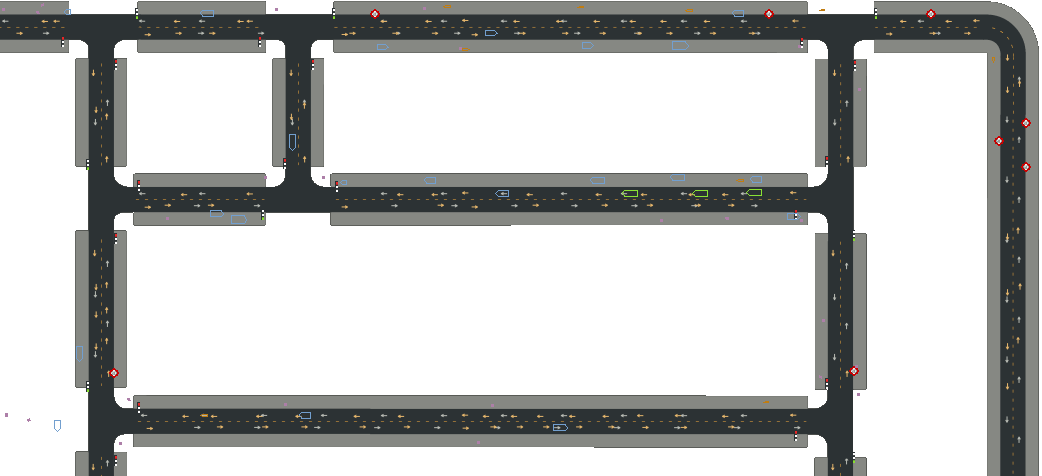
\includegraphics[width=1\linewidth]{98_images/evaluation_scene_topview_cropped}
	\caption[Top-View of the Simulation Environment used for Evaluation]{Schematic Top-View of an exemplary CARLA Simulation Environment used for Evaluation (\textit{Town01}). Green boxes indicate ego cars, blue boxes correspond to other, non-"'player"' vehicles.}
	\label{fig:carla_scene_topview}
\end{figure}

For all following tests, the fixed parameter values listed in \cref{tab:perception_evaluation:constant_parameters} are used. In addition to these, three further parameters are involved, which are varied across the three different test sets accordingly. 

\begin{itemize}
	\item \texttt{N\_VEHICLES} ($p_1$): The number of (communicating) ego vehicles to be used in an experiment. Fixed to $p_1 = 6$ for parts 1 and 3, varied wihtin $p_1 \in \{1, 3, 6\}$ for part 2.
	\item \texttt{DECAY\_FACTOR} ($p_2$): The factor to be used for decaying ("'down-weighing"') older observations during fusion. Fixed to $p_2 = 0.14$ for parts 1 and 2 and varied within $p_2 \in \{0.05, 0.08, 0.11, 0.14\}$ for part 3.
	\item \texttt{SEED} ($p_3$): Random seed used to initialize pseudo-randomness for reproducible start- and destination point generation. Fixed to $p_3 = 4$ for part 3 and varied within $p_3 \in \{4, 8, 16\}$ for all other experiments.
\end{itemize}

In each of the following three experiments, every scene setup is run five times for every parameter combination. That is, for the first part, $k_1 = |\textit{range}(p_3)| * 5 = 15$ tests are instantiated. Analogously, $k_2 = |\textit{range}(p_1)| * |\textit{range}(p_3)| * 5 = 45$ and $k_3 = |\textit{range}(p_2)| * 5 = 15$ runs are performed for parts 2 and 3 respectively.
\par
\bigskip

\subsubsection{Data Collection}
As mentioned before, every ego vehicle records both its local and – in the case of CP being enabled – its received fused observations. Observations are dumped to a file to be then used in a subsequent, offline (i.e. after the simulation has finished) analysis. \textbf{Offline analysis}, as opposed to computing evaluation scores online and in "'real time"' during the simulation, is necessary out of performance reason, as these computations would dramatically slow down the simulation. Alongside the ego vehicles themselves, an additional small program is run during the simulation, that is responsible for retrieving the actual, true obstacle position from the simulator. These are recorded to a file as well to be later used as ground truth measurements for comparison in the analysis. An important thing to note is that, out of technical reasons, only \textit{occupied} cells are recorded, but not \textit{free} ones. Accordingly, this evaluation only considers \textbf{true positives} and \textbf{false negatives} with regard to \textit{occupied}. This means that it can be distinguished between an occupied cell being observed correctly or not, while cells, that are \textit{free} in the ground truth data, are not included in the score.
\par
\bigskip

\subsubsection{Data Analysis \& Scoring}
The actual data analyses are subsequently performed in a downstream step using a separate Python script. It first reads in all observations from all ego vehicles and the previously mentioned ground truth data collector for a particular run.

As mentioned earlier, only an (occupied) occupancy cell's state will be considered, so an observation corresponds to a true or estimated cell state. Subsequently, the script essentially compares ground truth data to observations; once to those with CP enabled and again to the local ones only. Doing so all cells (= type 1 tiles, cf. \cref{subsec:concept_design:geographical_sharding}) are considered that are contained in the observer's current type 2 tile as well as in any of the neighboring type 2 tiles. \Cref{fig:eval_relevant_cells} in appendix \cref{subsec:appendix:texts:evaluation:perception_relevant_analyses} schematically depicts this in greater detail.

As a result of those comparisons, two scoring metrics – \textbf{recall (REC)} and \textbf{mean-squared error (MSE)} – are computed for every pair of true and estimated cell state. Eventually all values are aggregated to get a total scores for the entire run, i.e. all observations from all ego vehicles at every time stamp are combined. The meaning and definition of REC and MSE with regard to the current context is briefly explained in the following.
\par
\bigskip

Let $\vec{y}_i$ be a three-dimensional vector representing a cell's ternary (\textit{free}, \textit{occupied}, \textit{unknown}) state confidence, on which only one entry can be non-zero at a time. For instance, a 30 \% confidence for a cell state being \textit{occupied} could be expressed as $\vec{\hat{y}}_i = (0, 0.3, 0)$. Further, let a distinction be made between the true state vector $\vec{y}_i$ and its estimation (as part of a vehicle's observation) $\vec{\hat{y}}_i$ and let $Y$ and $\hat{Y}$ be the sets of all such true- and estimated state vectors respectively. Then, the following definitions for total, accumulated recall and MSE can be given.

\begin{gather}
	\textit{MSE}(Y, \hat{Y}) = \frac{1}{n} \sum_{i=1}^{n} \vec{y}_i \cdot (\vec{y}_i - \vec{\hat{y}}_i)^2 \\
	\textit{REC}(Y, \hat{Y}) = \frac{1}{n} \sum_{i=1}^{n} -\textit{sgn}(\vec{y}_i \cdot (\vec{y}_i - \hat{y}_i) - 1)
\end{gather}

\textbf{Example:} Assume a grid that consists of only two cells, the first of which is occupied and the second is free. Moreover, consider two observers, each estimating the grid cells' states. In the example, $\vec{\hat{y}}_{i,j}$ denotes the i-th vehicle's observation of cell j, i.e. $\vec{\hat{Y}}_i$ are all observations from vehicle i.

\begin{gather*}
	\vec{y}_1 = \begin{pmatrix}0 \\ 1 \\ 0 \end{pmatrix} \text{,\ } \vec{y}_2 = \begin{pmatrix}1 \\ 0 \\ 0 \end{pmatrix} \text{,\ }
	\hat{Y}_1 = \begin{pmatrix}
	0 & 0.5 \\
	0.8 & 0 \\
	0 & 0
	\end{pmatrix} \text{,\ }
	\hat{Y}_2 = \begin{pmatrix}
	0 & 0 \\
	0.6 & 0 \\
	0 & 0.9
	\end{pmatrix} \\
	\textit{MSE}(Y, \hat{Y}) = \frac{1}{4} (\begin{pmatrix}0 \\ 1 \\ 0 \end{pmatrix} \cdot \begin{pmatrix}0 \\ 0.2 \\ 0 \end{pmatrix}^2 + \text{...} + \begin{pmatrix}1 \\ 0 \\ 0 \end{pmatrix} \cdot \begin{pmatrix}1 \\ 0 \\ -0.9 \end{pmatrix}^2) = \frac{1}{4} (0.2^2 + \text{...} + 1^2) = 36.25 \% \\
	\textit{REC}(Y, \hat{Y}) = \text{...} = \frac{1}{4} (-\textit{sgn}(0.2-1) - \text{...} -\textit{sgn}(1-1)) = \frac{1}{4} (1+1+1-0) = 75 \%
\end{gather*}

\subsubsection{Test Setup}
As a test setup, the same physical machines are used as in \cref{subsec:evaluation:performance_evaluation:methodology}. The first machine runs the Carla simulator and all backend components, i.e. message broker and Talky fusion node. For the configurations comprising only one or three ego vehicles, all client-side components, i.e. simulation client and Talky client, are run on the second machine. In the last configuration involving six ego cars, four of them are run on machine 2 and the remaining two out of six on machine 1.

\subsection{Results}
\label{subsec:evaluation:perception_evaluation:results}
It was mentioned before that the first step involves evaluating whether perception quality can be improved through the proposed CP system. Therefor, different simulation scenes were instantiated and repeatedly run for a total of 15 experiments. Given the recorded data, CP was "'virtually"' turned on and off during evaluation to measure the difference with respect to MSE and recall. This yielded the results depicted in \cref{fig:perception_evalutation_scores_1}.

\begin{figure}
	\centering
	\begin{subfigure}[b]{1\textwidth}
		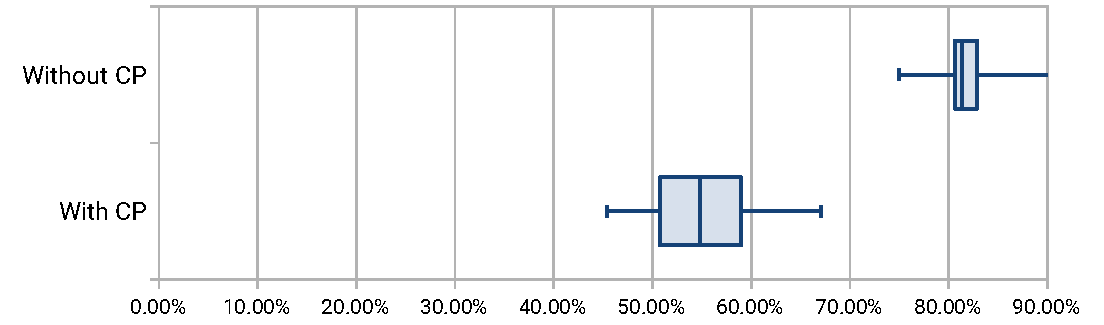
\includegraphics[width=1\linewidth]{98_images/eval_boxplot_2}
		\caption{Average MSE for \texttt{N\_VEHICLES = 6} (lower is better)}
		\label{fig:eval_boxplot_2} 
	\end{subfigure}
	
	\begin{subfigure}[b]{1\textwidth}
		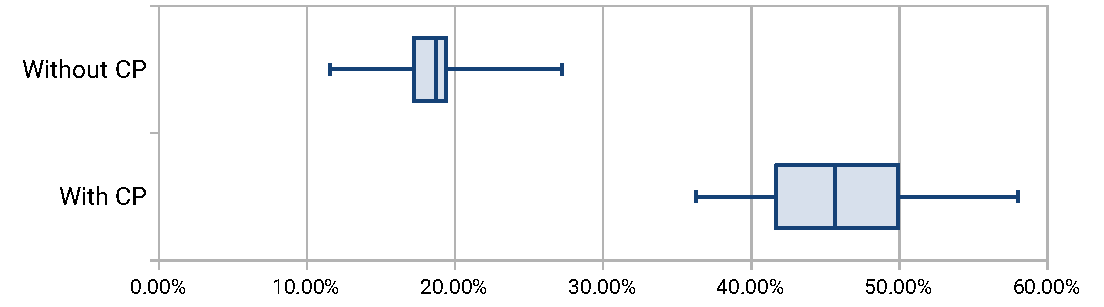
\includegraphics[width=1\linewidth]{98_images/eval_boxplot_3}
		\caption{Average recall for \texttt{N\_VEHICLES = 6} (higher is better)}
		\label{fig:eval_boxplot_3}
	\end{subfigure}

	\begin{subfigure}[b]{1\textwidth}
		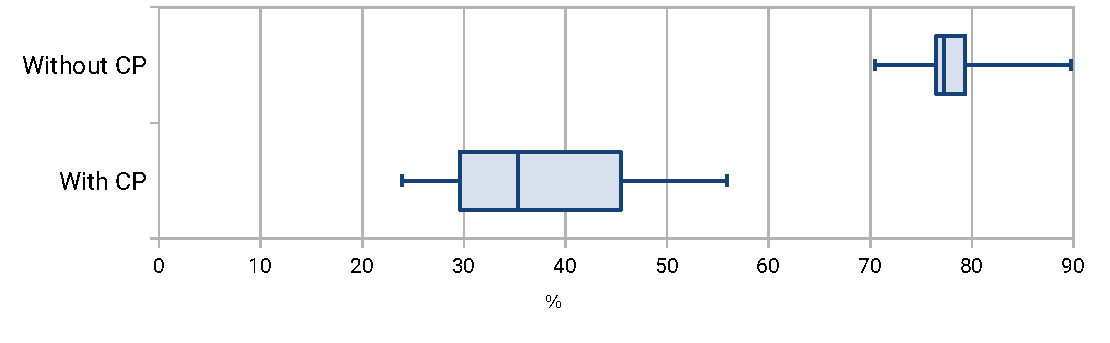
\includegraphics[width=1\linewidth]{98_images/eval_boxplot_1}
		\caption{Average percentage of \textit{unknown} cells for \texttt{N\_VEHICLES = 6} (lower is better)}
		\label{fig:eval_boxplot_1}
	\end{subfigure}
	\caption{Perception Evaluation Scores – }
	\label{fig:perception_evalutation_scores_1}
\end{figure}

It can be clearly seen that both scores are higher with cooperative perception, i.e. with the ego vehicles communicating and exchanging their environment state representations. Looking at arithmetic mean for recall and MSE in the above scenario, it can be found that $\Delta \diameter_{MSE} = -27.13 \%$ and $\Delta \diameter_{REC} = 27.73 \%$. In addition, when looking at the average number of unknown cells, that could potentially have been observed, one finds that $\Delta \diameter_{unkown} = -41.11 \%$, i.e. $\sim$ 40 \% more cells are "'unveiled"' for each vehicle with CP.
\par
\bigskip

After an actual improvement in perception quality through CP could be observed, the following additional results were obtained from viewing that improvement in relation to two parameters, the number of employed connected vehicles and the temporal decay factor. Since the absolute recall and MSE values for two different configurations of \texttt{N\_VEHICLES} can NOT be compared for various reasons, only relative changes are considered in the following. In other words, given exemplary values of $\textit{MSE}_{n=6, CP}(Y_1, \hat{Y}_1) = 50 \%$ and $\textit{MSE}_{n=3, CP}(Y_2, \hat{Y}_2) = 45 \%$ does NOT imply that six vehicles are 5 \% better than three. Conversely, one can instead draw such a conclusion when comparing relative differences between with and without CP, e.g. $\Delta \diameter_{MSE,n=6} = -10 \%$ and $\Delta \diameter_{MSE,n=2} = -5 \%$.

\begin{figure}
	\centering
	\begin{subfigure}[b]{0.49\textwidth}
		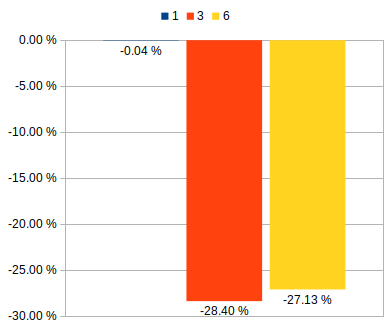
\includegraphics[width=1\linewidth]{98_images/eval_barplot_nvehicles}
		\caption{Average MSE change due to CP for different \texttt{N\_VEHICLES}}
		\label{fig:eval_barplot_1} 
	\end{subfigure}
	\begin{subfigure}[b]{0.49\textwidth}
		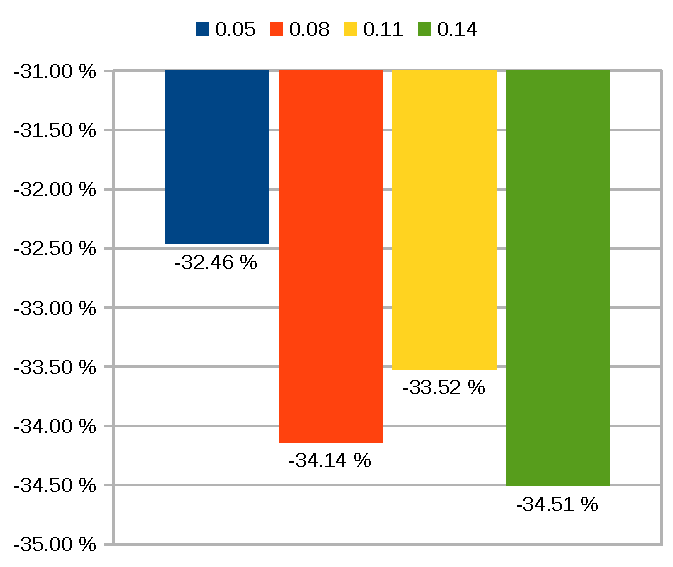
\includegraphics[width=1\linewidth]{98_images/eval_barplot_decay}
		\caption{Average MSE change due to CP for different \texttt{DECAY\_FACTOR}}
		\label{fig:eval_barplot_2}
	\end{subfigure}
	\caption{Perception Evaluation Scores – Part 2}
	\label{fig:perception_evalutation_scores_2}
\end{figure}

\Cref{fig:perception_evalutation_scores_2} (left) shows the results for different configurations when varying the number of employed connected vehicles, or observers in general. First, it becomes clear that there is no quality improvement at all between CP being turned on and off when using only one vehicle. This is plausible, since the key point of cooperative perception is to benefit from other traffic participant's observations in addition to one's own. Moreover, no significant increase or decrease in MSE can be perceived when varying the number of network participants between three and six. With regard to the temporal decay factor, a value of $0.14$, i.e. a comparatively "'aggressive' down-weighing of old observations, seems to yield the best results. However, since the differences are only marginal, one might not speak of a significant impact of \texttt{DECAY\_FACTOR} on the final score, at least in these brief experiments.

\subsection{Discussion \& Conclusion}
\label{subsec:evaluation:perception_evaluation:discussion_conclusion}
The previous evaluation clearly unveiled that the averasge, overall perception quality can be improved through cooperation, specifically through the use of the presented CP system. Similar to what Chen et al. \cite{Chen2019} discovered for their CP system, we found that both a vehicle's perception range or field of view as well as the average confidence for single measurements can be increased. In our experiments, we discovered an average improvement in total, accumulated mean squared error of $\sim$ 27\% and a $\sim$ 27\% better recall likewise. In addition, we found that $\sim$ 41\% more potentially observable cells were actually observed, i.e. they were assigned a state estimation other than \textit{unknown}. As a result of briefly investigating the total MSE improvement as a function of the number of connected vehicles and the decay factor used for fusion, we did not find a significant impact of neither of both.

While we experimentally showed the general suitability of the proposed system to increase overall end-to-end perception quality, further evaluation with a greater range of different scenarios and parameter settings is needed in order to gain more extensive insights about conceptual strength and weaknesses and about limitation of the current prototype implementation. 